\chapter{Verwendete Technologien}\label{cha:theoretical-background}


\section{Visual Studio}
Visual Studio ist eine Entwicklungsumgebung von Microsoft. Sie wird verwendet um Computerprogramme sowie Webseiten, Webapps, Webservices und mobile Apps herzustellen. Die aktuellste Version des Programmes unterstützt eine vielzahl von Programmiersprachen: Visual Basic, .NET, C, C++, C++/CLI, C++/CX, C\#, F\#, SQL Server, TypeScript, Python, HTML, JavaScript und CSS.
Weiters verfügt Visual Studio über einen Code editor mit IntelliSense(unterstützt den Programmierer mittels Vervollständigung des Codes).

\section{C-Sharp}
C\# ist eine objektorientierte Programmiersprache. Sie wurde von Microsoft entwickelt ist jedoch mittlerweile Plattform unabhängig. Sie unterstützt zahlreiche Funktionen wie Lambda Expressions, Delegates, Enumerationen und auch einem direkten Speicherzugriff. Außerdem werden generische Methoden und Typen von C\# unterstützt.


\section{MVC}
Model-View-Controller ist ein Design-Muster für die Trennung einer Software in 3 miteinander verbundene Teile. Das MVC-Muster wurde entwickelt um eine Wiederverwendung von Objektcode zu ermöglichen. Das Muster soll die Entwicklungszeit von Anwendungen mit Benutzeroberflächen stark  reduzieren. 
Die 3 Hauptkomponenten die bei hier verwendet werden sollen stecken schon im Namen und zwar: 
\begin{itemize}

\item Model: Ein Model ist eine simple Klasse und stellt das einfachste Element in MVC dar. Das Modell enthält die darzustellenden Daten. Es ist von View und Controller unabhängig. Es bedarf keiner Ableitung oder anderer Implementierung und ist im Prinzip ein Datencontainer. Die Models befinden sich in dem Order /Models. Wobei die Klassen ohne weiteres in eine Klassenbibliothek ausgelagert werden können. In einem Model befinden sich nichts anderes als Properties – Properties, die das Element bzw. die Daten darstellen, die für die Präsentation bestimmt sind. Ebenfalls kann beim Senden von Daten (POST) von einer View zum Controller eine Model-Klasse verwendet werden. Dabei wird der Controller-Action das Model als Parameter übergeben. Das Mappen zwischen POST-Parametern und Model findet über das Model-Binding statt.

\item View: Sie kennt sowohl ihren Controller als auch das Model, dessen Daten sie präsentiert, ist aber nicht für die Weiterverarbeitung der vom Benutzer übergebenen Daten zuständig. Im Regelfall wird die View über Änderungen von Daten im Model mithilfe des Observers unterrichtet und kann daraufhin die aktualisierten Daten abrufen. Die View kann sich selbst aktualisieren, kennt das Model und ist dort registriert.
Es gibt außerdem noch spezielle Views, die von allen Controllern bzw. allen Views verwendet werden können, die sogenannten Partial Views.

\item Controller: Der Controller ist Verantwortlich für die Interaktion des Benutzers mit der Anwendung und für die Steuerung der Verarbeitung zwischen Model und View (Ablauf, Datenverarbeitung, entscheidet welche Views aufgerufen werden)
Er kann den Kontext für verschiedene Models und Views darstellen und bestimmt die Möglichkeiten, mit denen die Benutzungsschnitstelle auf Benutzereingaben reagieren kann.
Er ist nichts anderes als eine Klasse, die sich von System.Mvc.Controller ableitet. 
Eine Controller besteht meist aus mehreren Aktionen, die HTTP-Methoden, wie GET und POST, darstellen. Im einfachsten Falle übernimmt der Controller die Aufgabe des Business Layers und verarbeitet Daten. Dies kann ein Serviceaufruf, eine Datenbankabfrage, Dateihandling oder einfach auch nur ein Verarbeiten von Strings oder Zahlen sein.
\end{itemize}
Es verwandelt eine Webanwendung in eine wartbare, modulare und effizient entwickelte Anwendung. 
Anwendungsaufgaben in Models, Views und Controllers zu teilen macht Deine Anwendung sehr schlank. 
Neue Features sind einfach hinzugefügt, alte Features schnell in einer neuen Oberfläche verpackt. 
Die modular und unterteilte Logik erlaubt Entwicklern und Designern gleichzeitig an der Anwendung zu arbeiten. 
Dies beinhaltet ebenso die schnelle Entwicklung eines ersten Prototyps. 
Dadurch ist es ebenso möglich einen Teil der Anwendung zu verändern, ohne einen anderen Teil zu beeinflussen.
\begin{figure}[H]
\begin{center}
	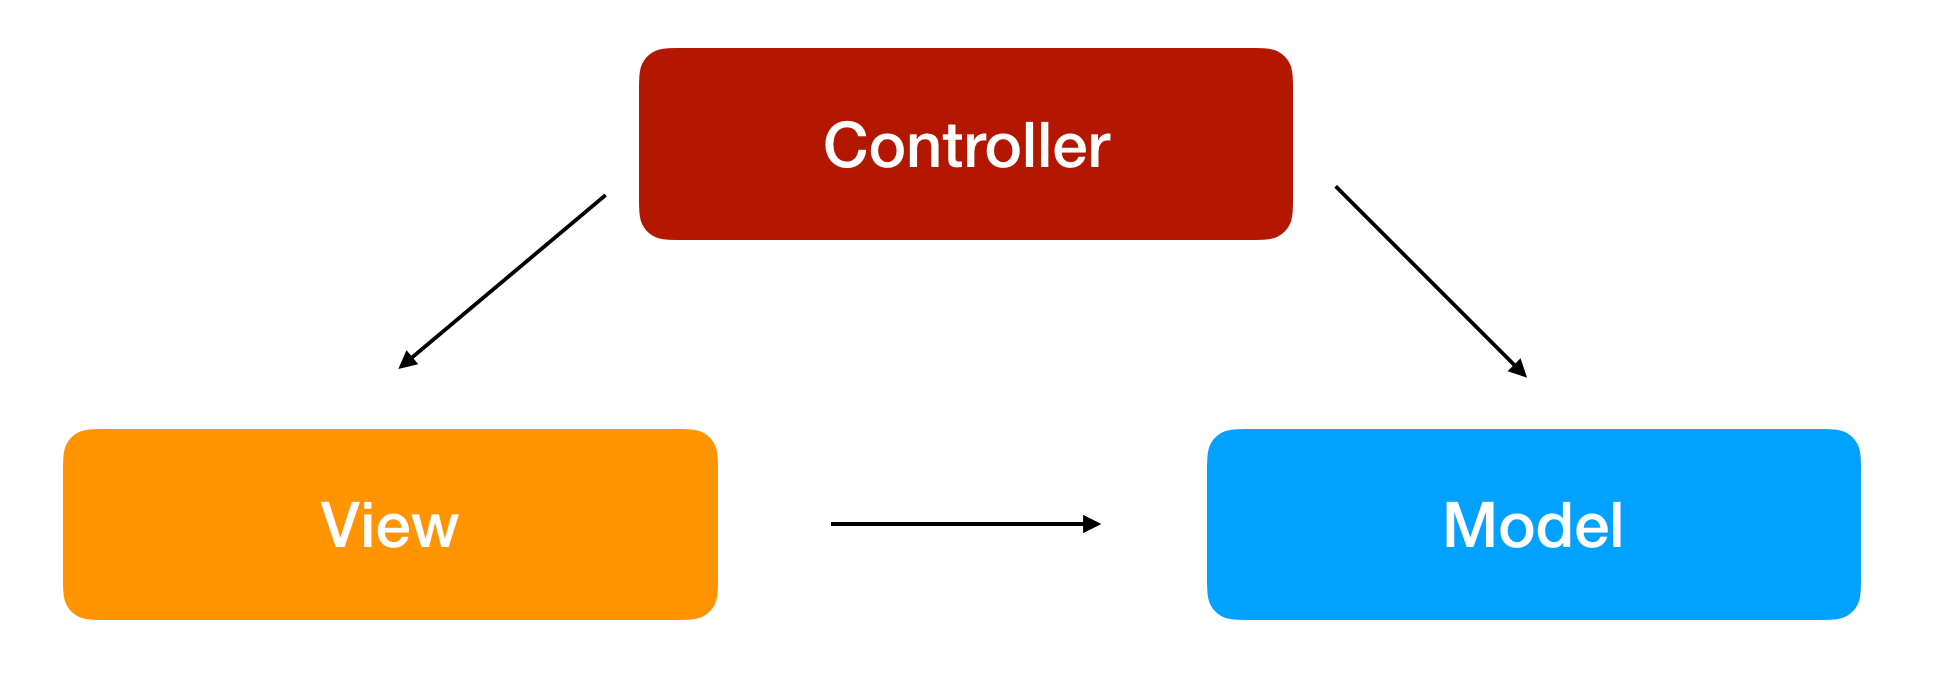
\includegraphics[scale=.4]{images/MVC.png}
\end{center}
	\caption{Model-View-Controller Konzept}
	\label{fig:sample}
\end{figure}

\section{HTML}
Hypertext Markup Language oder auch HTML ist die Standardsprache für das erstellen von Webseiten und Web Applikationen. Gemeinsam mit CSS und Javascript gehört HTML zu den Eckpfeiler Technologien vom World Wide Web.
Die meisten HTML-Elemente starten und enden jeweils mit einem Tag. Der Starttag beginnt immer mit dem Zeichen <. Nach dem < folgt der Elementname und dann wird der Starttag mit dem > Zeichen geschlossen. Nach dem Elementnamen können auch noch Attribute eingefügt werden.
Der Endtag startet immer mit den Zeichen </, dann dem Elementnamen und endet mit einem > Zeichen.

\section{CSS}
Cascading Style Sheets ist eine style sheet Sprache welche gemeinsam mit HTML und DOM zu den Kernsprachen des World Wide Web gehört.
Sie wird meist verwendet um einen visuellen Stilauf Webseiten festzulegen.

\subsection{Media Query}
Media Query ist eine Technik die es seit CSS3 gibt.
Sie verwendet die @media Regel um einen bestimmt Block von Css Eigenschaften zu verwenden, wenn eine bestimmte Bedingung erfüllt wurde.

\begin{lstlisting}
@media only screen and (max-width: 600px) {
    body {
        background-color: black;
    }
}
\end{lstlisting}

\section{Bootstrap}
Bootstrap ist ein freies web framework für das designen von Webseiten und Webapps. Es enthält HTML- und CSS basierte Design Vorlagen für Typografie, Buttons, Tabellen, Grid-Systeme, Formulare, Navigations- und andere Elemente. Außerdem kann man optional auch JavaScript Erweiterungen verwenden.

\subsection{Grid-Systeme}
Die Bootstrap Grid-Systeme sind mobile responsive was bedeutet das sie ihr Layout auf die größe des Gerätes anpassen. Würde man das unten angefürte Beispiel auf dem Computer aufrufen würden 3 gleich große nebeinander gestellte Spalten angezeigt werden, am Handy würde sich dies platztechnisch nicht ausgehen deshalb werden diese 3 Spalten automatisch untereinander gestellt.

\begin{lstlisting}
<div class="row">
  <div class="col-sm-4">
  	Spalte 1
  </div>
  <div class="col-sm-4">
  	Spalte 2
  </div>
  <div class="col-sm-4">
  	Spalte 3
  </div>
</div>
\end{lstlisting}

\section{SMTP}
Simple Mail Transfer Protocol ist ein standard Internetprotokoll zur Übertragung von emails. SMTP wird vorrangig für das versenden von Mails benutzt, da zum Empfang von Mails andere Protokolle wie zum Beispiel POP3 oder IMAP verwendet werden.

\section{Base64}
Base64 ist eine Gruppe ähnlicher Binär zu Text Codierungsschemas, die Binärdaten in einem ASCII-Zeichenfolgenformat darstellen, indem sie in eine Radix-64-Darstellung übersetzt werden.